\section{Исследование методов организации процесса обработки данных в СЭД} \label{experiment}

Система электронного документооборота, как и любая другая система, может быть представлена в виде совокупности модулей, выполняющих различные функции. %Так как документооборот --- детерминированный процесс, каждый этап которого может быть детально расписан, можно рассматривать такие этапы в отдельности. 
Для каждого модуля исходя из особенностей его работы можно определить варианты реализации. Наибольший интерес будут представлять следующие модули:
\begin{itemize}
	\item модуль обеспечения совместной работы пользователей;
	\item модуль обнаружения ошибок при обработке документа;
	\item модуль хранения истории внесённых изменений.
	% \item модуль авторизации.
\end{itemize}
Остальные модули (передачи данных, разграничения доступа, защиты хранилища от несанкционированного доступа) реализуются стандартными методами и не представляют такого интереса.

\vspace{\baselineskip}
Для выбора реализации модулей СЭД в соответствии с показателями эффективности, которые будут описаны позднее, необходимо провести экспериментальное исследование существующих реализаций подобных модулей. Так как системы электронного документооборота д\'{о}роги и сложны в развёртывании, не все компании предоставляют демо-версии своих продуктов. Но и в случае наличия демо-версии довольно сложно её получить и оценить параметры (часто вместо демо-версии предоставляется презентация, а также отсутствует доступ к отдельным модулям системы). Существует и ещё один фактор, затрудняющий сложность проведения эксперимента: так как СЭД является системой массового обслуживания, для её объективного тестирования необходимо провести множество однотипных испытаний, включающих в себя работу нескольких испытуемых (пользователей СЭД) в течение длительного времени.

\vspace{\baselineskip}
С учётом всех вышеизложенных ограничений было принято решение провести имитационное моделирвоание модулей СЭД в среде AnyLogic, приняв за описание моделей базовые принципы построения исследуемых модулей в различных реализациях.

\subsection{Модуль обнаружения ошибок при обработке документа} \label{research_feedback}

При обработке документов автоматизирвоанным способом существует возможность обнаружения ошибок на стадии редактирования, т.е. до отправки документа далее по цепочке обработки. В таком случае ошибка либо устраняется автоматически, либо создаётся новая задача на устранение ошибки тому же редактору, который допустил эту ошибку.

\vspace{\baselineskip}
Одной из разновидностей ошибки такого рода является некорректное обращение к полям документа. Стоит отметить, что речь здесь идёт не о метаданных, сопровождающих документ, а об информации, содержащейся непосредственно в документе. Например, для совместной работы, описанной в гл. \ref{research_competition}, таким обращением будет считаться попытка редактирвоания полей документа, обработкой которых уже занимается другой редактор.

\vspace{\baselineskip}
Для эксперимента были рассмотрены две схемы: одна --- <<классическая>>, без обнаружения ошибок такого рода (многие СЭД не предоставляют подобного сервиса, регулируя только поля метаданных, см. табл. \ref{table:products}), другая --- согласно описанной выше схеме, реализованная в описываемой разработке.

\vspace{\baselineskip}
На рис. \ref{img:feedback_old_scheme} представлена схема без автоматизированного обнаружения ошибок. Возврат на доработку при такой организации возможен, но осуществляется в ручном режиме: редактор, получивший на вход задания документ с ошибкой, отправляет его на переработку предыдущему редактору. Последний редактор в случае допуска ошибки получит неверный документ, на схеме приёмник таких результатов обозначен $sink$. Корректно обработанные заявки приходят в пункт $sink2$. Разветвления после обработчиков работают по вероятностному принципу с вероятностью обнаружения ошибки $P_{txt}'$.
 
\begin{figure}[h!]
  \centering
  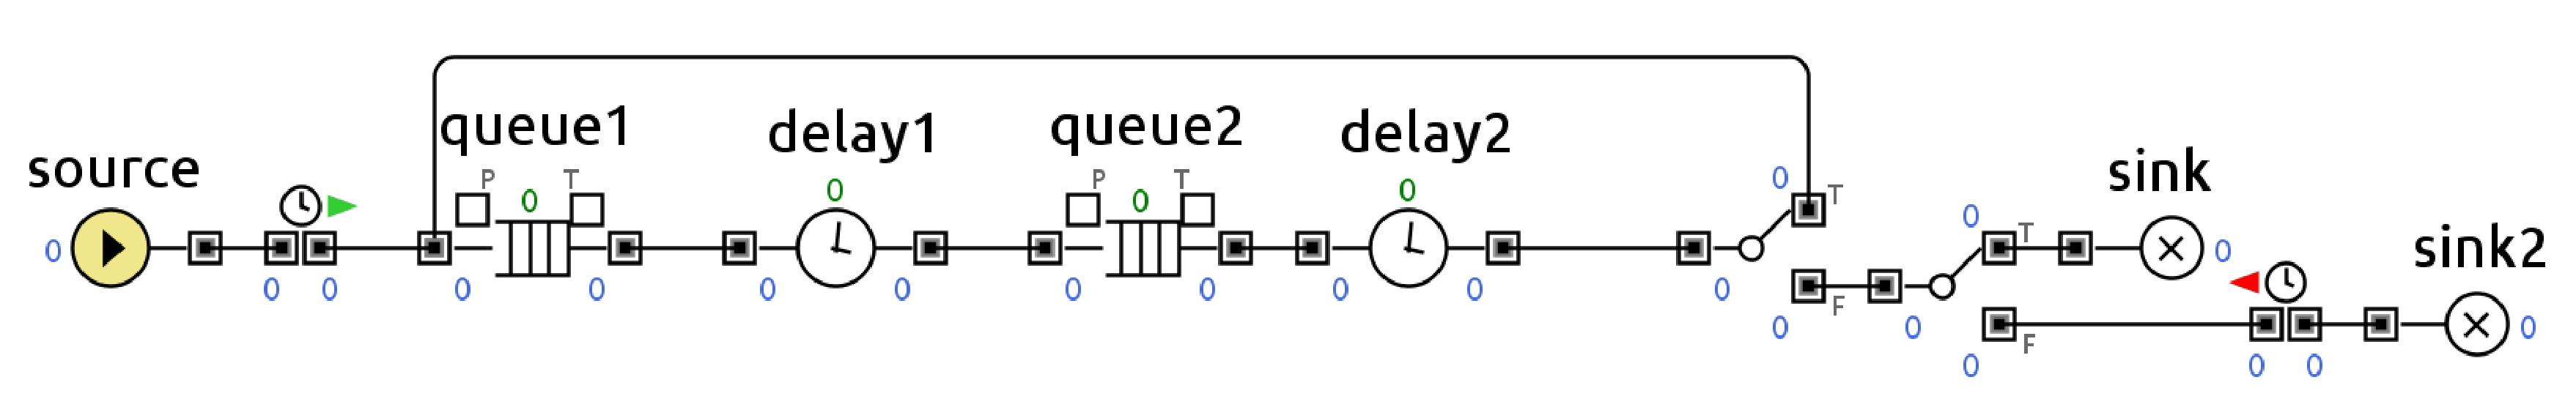
\includegraphics[width=1\textwidth]{feedback_old_scheme}
  \caption{Схема коррекции ошибок ручным методом}
  \label{img:feedback_old_scheme}
\end{figure}

\vspace{\baselineskip}
В данной схеме бъекты $source$ моделируют источники заявок (по одной заявке в полчаса), $queue$ --- персональные очереди заявок на обработку, $delay$ --- редакторов (время обработки заявки распределяется по нормальному закону со средним значением 25 минут, $\sigma=5$), $sink$ --- целевое хранилище, собирающее обработанные заявки.

\vspace{\baselineskip}
В случае автомтизированного обнаружения ошибок (рис. \ref{img:feedback_new_scheme}) задание на переработку генерируется автоматически для того редактора, который допустил ошибку. Таким образом, даже последний редактор в цепочке имеет возможность исправить допущенную ошибку перед публикацией документа.

\begin{figure}[h!]
  \centering
  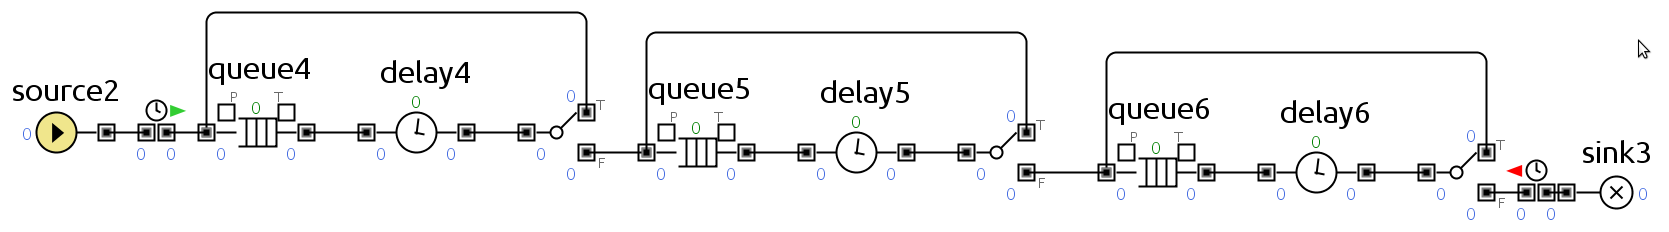
\includegraphics[width=1\textwidth]{feedback_new_scheme}
  \caption{Схема коррекции ошибок автоматизированным методом}
  \label{img:feedback_new_scheme}
\end{figure}

\vspace{\baselineskip}
Одним из показателей эффективности метода организации процесса обработки документов является число корректно обработанных заявок. В процессе эксперимента заявки генерировались по одной за полчаса реального времени, был промоделирован один рабочий день (с 9:00 до 18:00). Результат моделирования представлен на рис. \ref{img:feedback_done}.

\begin{figure}[h!]
  \centering
  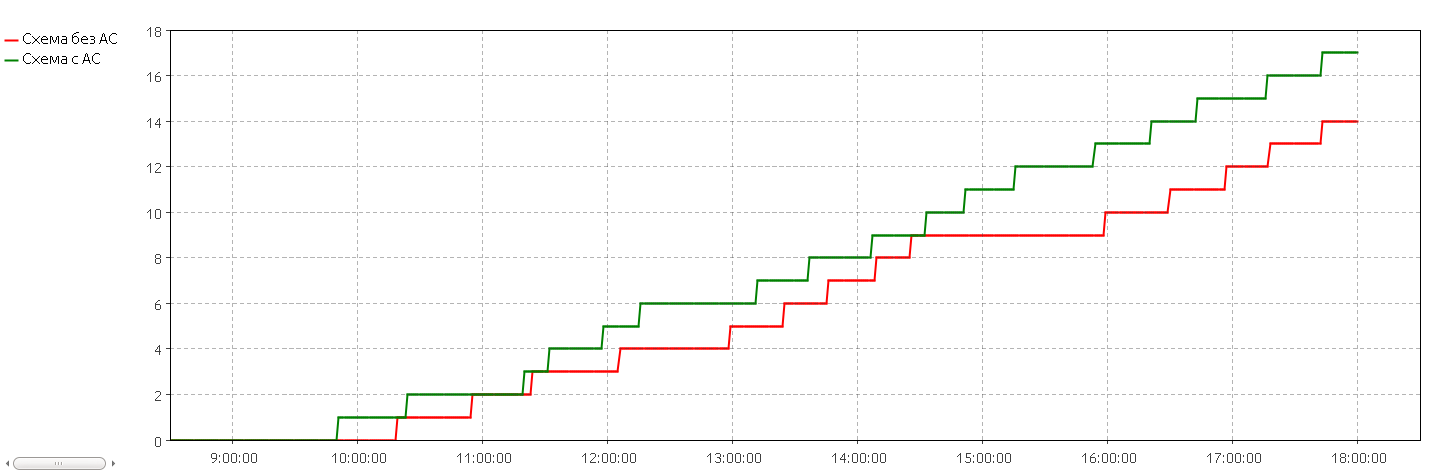
\includegraphics[width=1\textwidth]{feedback_done}
  \caption{Число обработанных заявок в схемах с обратной связью}
  \label{img:feedback_done}
\end{figure}

\vspace{\baselineskip}
Как видно из рисунка, схема с автоматизирвоанным обнаружением ошибок позволяет обработать больше заявок за ограниченный промежуток времени. Также можно заметить, что частота, с которой заявкам присваивался статус <<корректно обработанная>>, выше в схеме с АС. Это позволяет предположить, что среднее время обработки одной заявки при такой организации меньше, чем при ручном обнаружении ошибок. Данная гипотеза подтверждается графиком, приведённым на рис. \ref{img:feedback_mean}.

\begin{figure}[h!]
  \centering
  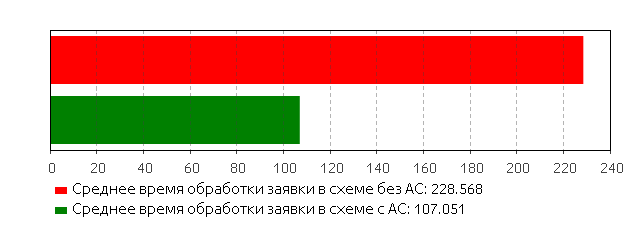
\includegraphics[width=1\textwidth]{feedback_mean}
  \caption{Среднее время обработки одной заявки в схемах с обратной связью}
  \label{img:feedback_mean}
\end{figure}

\vspace{\baselineskip}
Уменьшение времени обработки заявки происходит за счёт того, что в случае необходимости исправления ошибки над документом работает один редактор из цепочки (тот, который допустил ошибку), а не все.
% Более того, среднее время обработки заявки в схеме без АС можно считать заниженным, т.к. в нём не учтено время поиска ошибки, а сама вероятность её обнаружения оценена довольно высоко --- наравне с АС. 

\vspace{\baselineskip}
Таким образом, для снижения времени обработки заявок целесообразно использовать систему автоматического обнаружения ошибок.				% Возврат на доработку
\subsection{Модуль обеспечения совместной работы пользователей} \label{research_competition}

При совместной конкурентной работе пользователей в системе электронного документооборота существует проблема синхронизации вносимых изменений. Так, два редактора, работая над одним документом (каждый со своим набором задач), во время внесения изменений блокируют работу друг друга, так как документ в рассматрвиаемом контексте --- ограниченный ресурс. В один момент времени возможно только одно внесение изменений, это показано на рис. \ref{img:graph_oldscheme}.
\begin{figure}[h!]
  \centering
  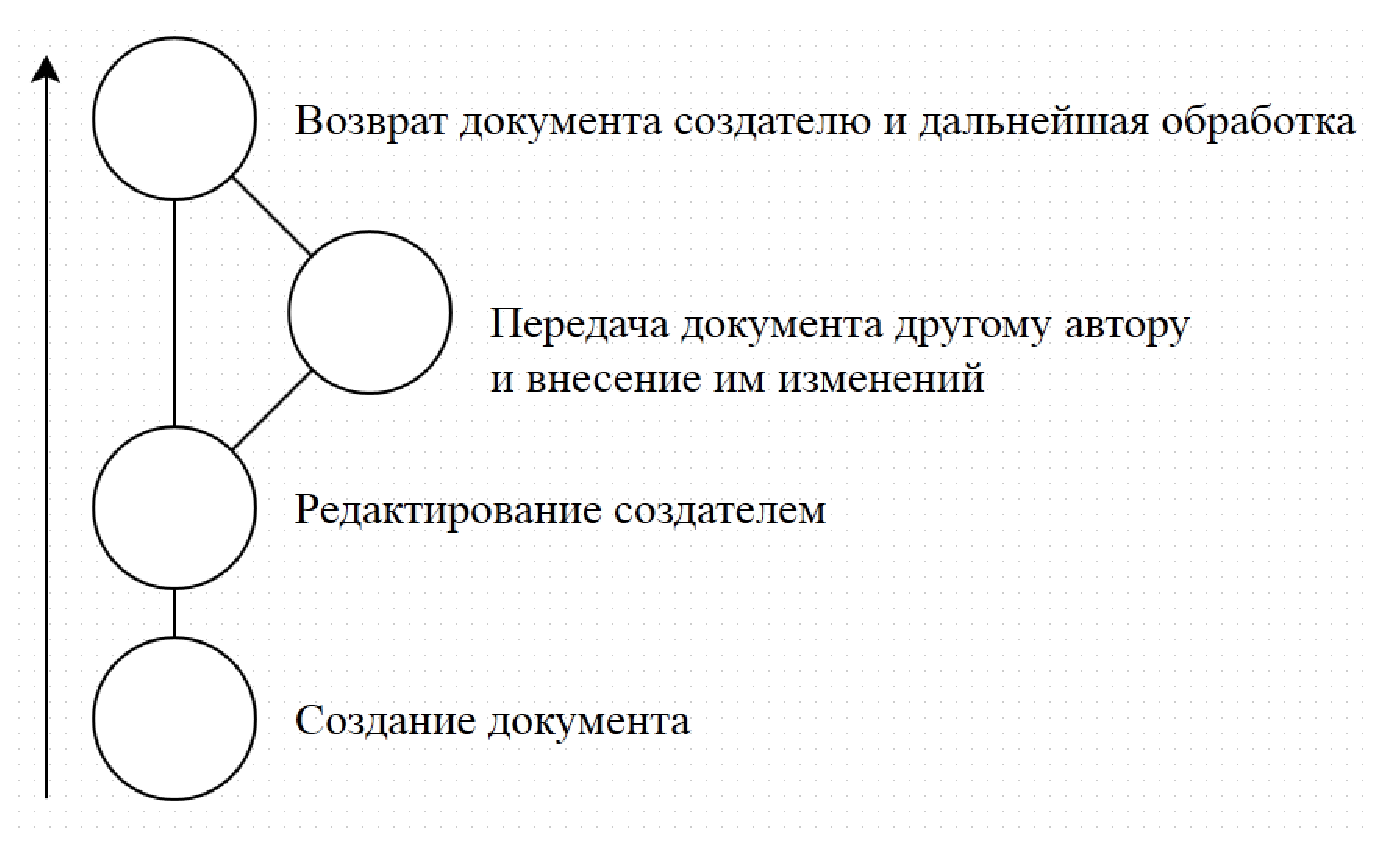
\includegraphics[width=0.7\textwidth]{graph_oldscheme}
  \caption{Схема конкурентной обработки документа с блокировкой}
  \label{img:graph_oldscheme}
\end{figure}

\vspace{\baselineskip}
Схема такой модели в среде AnyLogic представлена на рис. \ref{img:competition_old_scheme}.
\begin{figure}[h!]
  \centering
  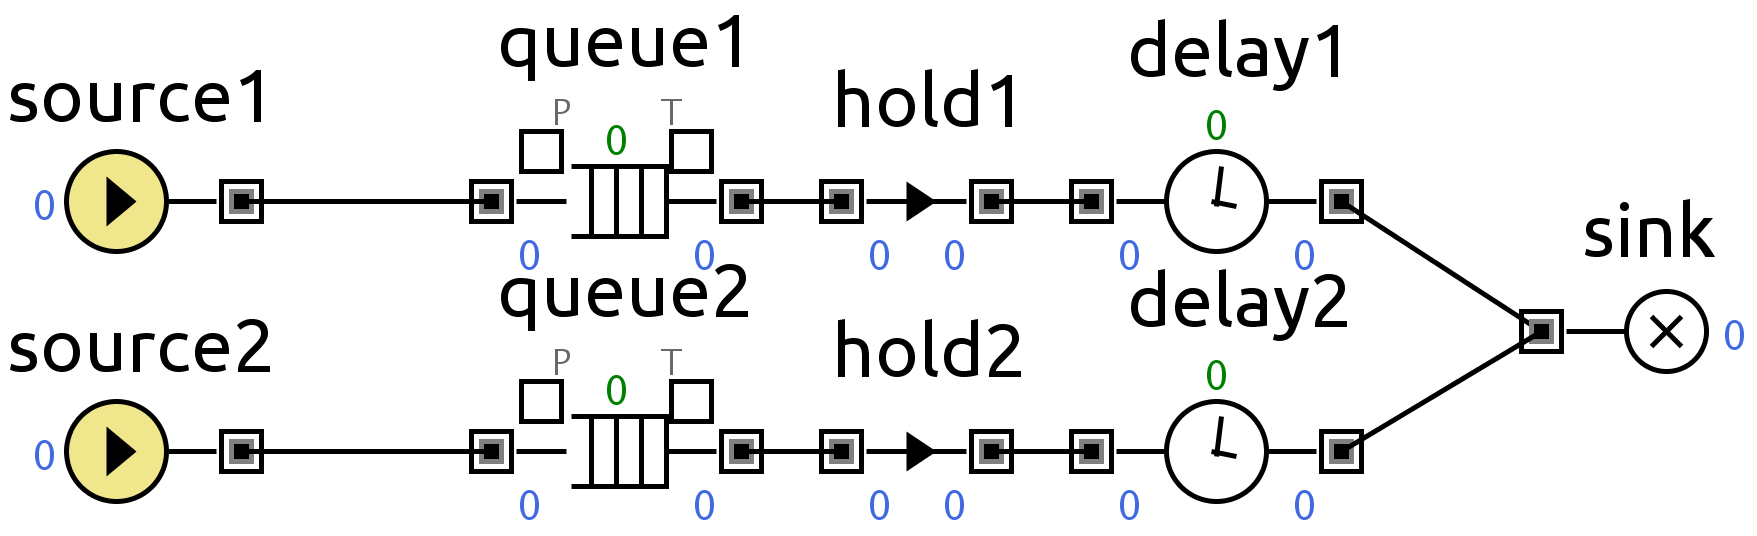
\includegraphics[width=0.7\textwidth]{competition_old_scheme}
  \caption{Модель обработки документа с блокировкой в среде AnyLogic}
  \label{img:competition_old_scheme}
\end{figure}

Здесь объекты $source$ моделируют источники заявок (по одной заявке в полчаса), $queue$ --- персональные очереди заявок на обработку, $hold$ --- элемент, блокирующий работу редактора (когда работает первый редактор, второй блокируется, и наоборот), $delay$ --- редакторы (время обработки заявки распределяется по нормальному закону со средним значением 25 минут, $\sigma=5$), $sink$ --- целевое хранилище, собирающее обработанные заявки.

\vspace{\baselineskip}
Альтернативой является такая схема организации обработки документов, при которой разрешено одновременное внесение изменений в документ, что справедливо для разрабатываемой системы --- см. рис. \ref{img:graph_newscheme}. Это становится возможным благодаря регистрации не состояний документа, а вносимых в него изменений в виде разницы текущего и предыдущего состояний. Пример такой разностной записи показан на рис. \ref{img:git_patch}.

\begin{figure}[h!]
  \centering
  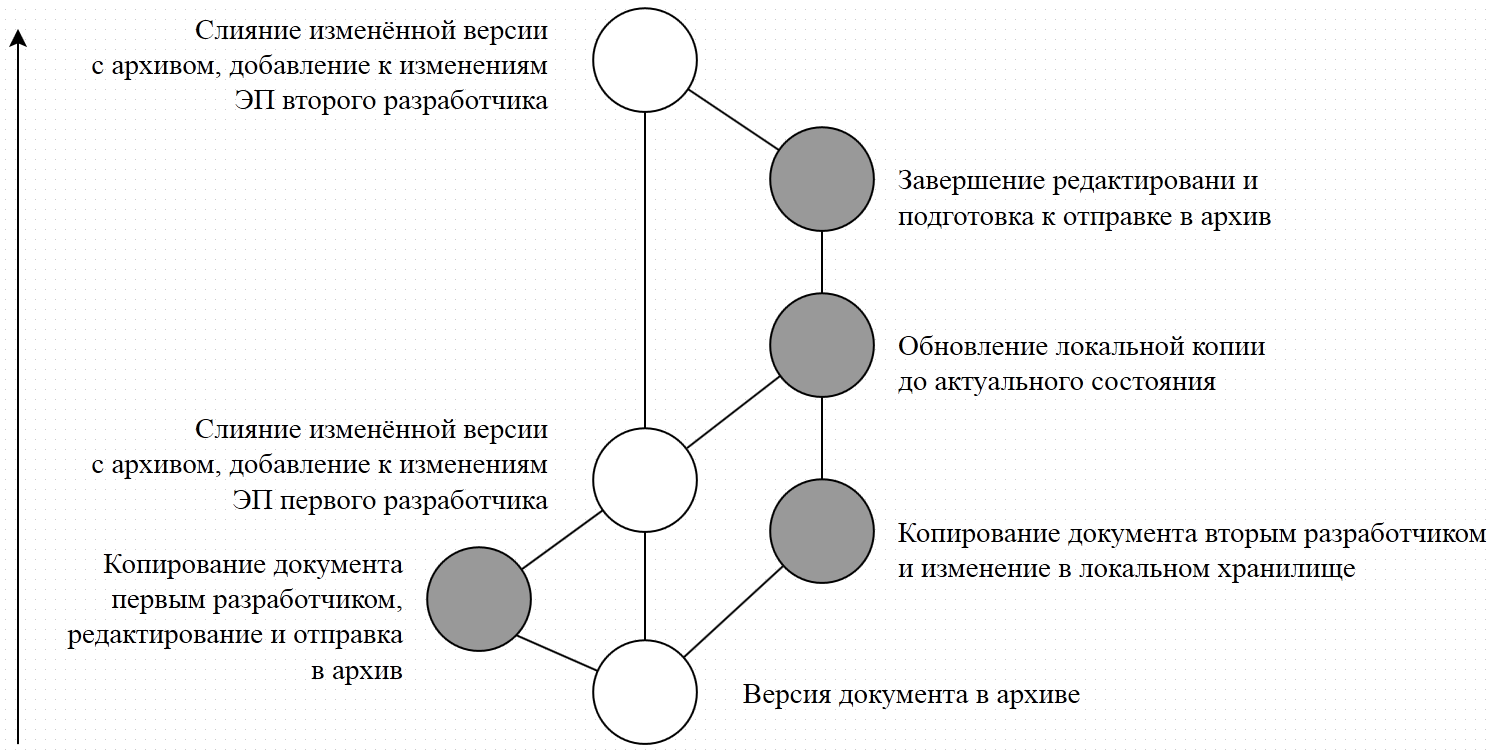
\includegraphics[width=1\textwidth]{graph_newscheme}
  \caption{Схема конкурентной обработки документа без блокировки}
  \label{img:graph_newscheme}
\end{figure}

\begin{figure}[h!]
  \centering
  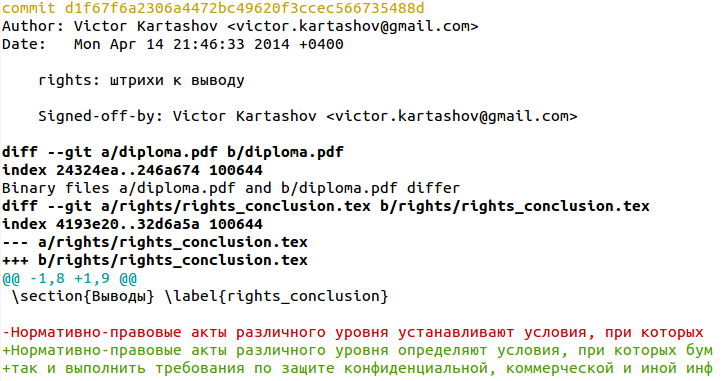
\includegraphics[width=0.8\textwidth]{git_patch}
  \caption{Пример описания состояния документа в виде разностной записи}
  \label{img:git_patch}
\end{figure}

Подобная структура может быть представлена в удобном для восприятия человеком виде, как показано на рис. \ref{img:git_meld}.
\begin{figure}[h!]
  \centering
  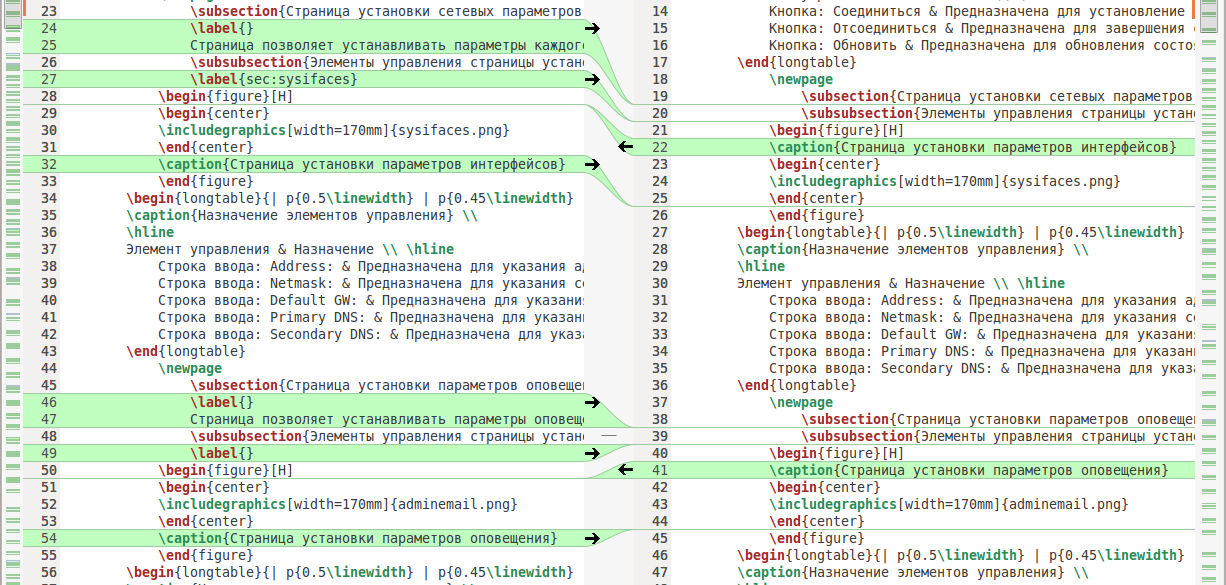
\includegraphics[width=1\textwidth]{git_meld}
  \caption{Пример представления разностной записи в виде постраничного сравнения}
  \label{img:git_meld}
\end{figure}

Данная реализация позволяет не только сократить объём хранимых данных, но и реализовать вышеописанную схему, ведь при таком подходе одновременное внесение изменений несколькими редакторами рассматривается не как изменение одного документа, а как создание набора новых записей. Результирующий документ получается путём последовательного применения таких <<патчей>> к исходному документу.

\vspace{\baselineskip}
Схема этой модели в среде AnyLogic представлена на рис. \ref{img:competition_new_scheme}.

\begin{figure}[h!]
  \centering
  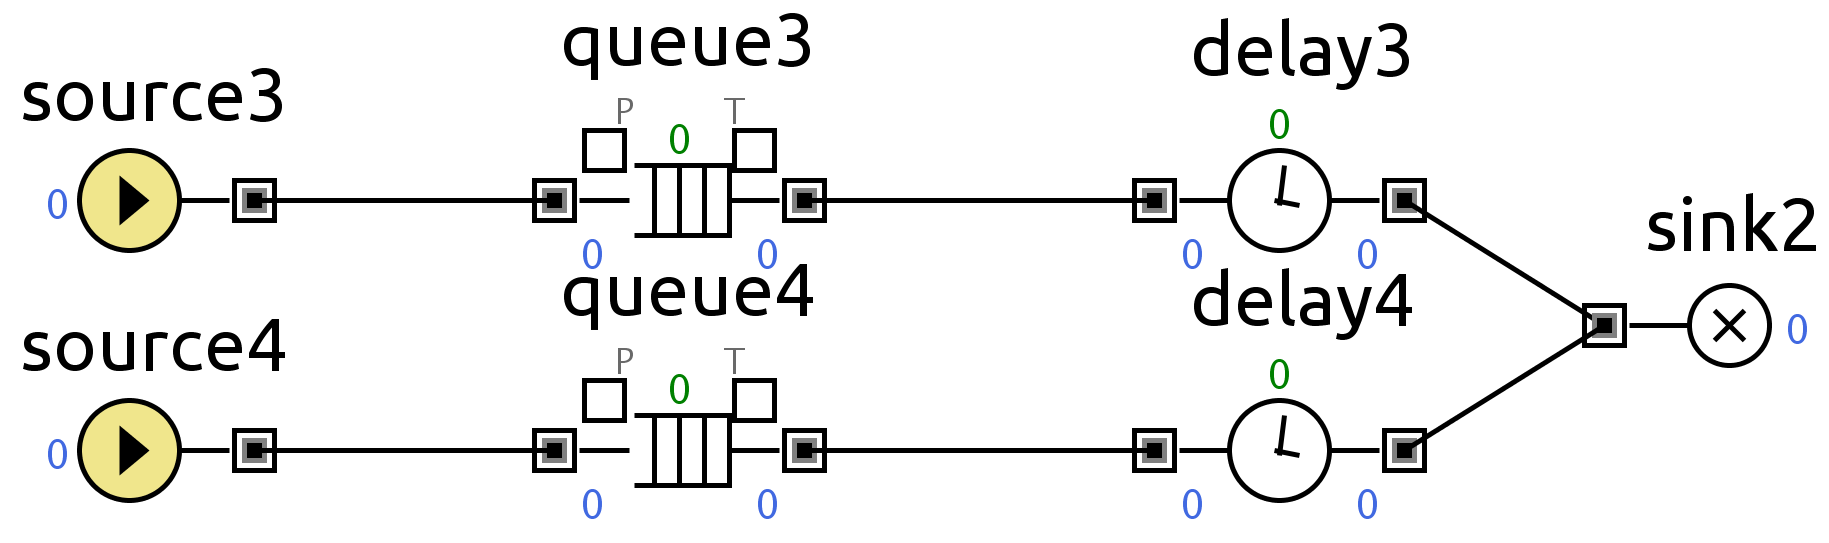
\includegraphics[width=0.7\textwidth]{competition_new_scheme}
  \caption{Модель обработки документа без блокировки в среде AnyLogic}
  \label{img:competition_new_scheme}
\end{figure}

\vspace{\baselineskip}
Элементы на этой схеме совпадают с элементами схемы рис. \ref{img:competition_old_scheme}, однако здесь отсутствуют блоки $hold$, а время обработки заявки распределяется по нормальному закону со средним значением 30 минут, $\sigma=6$ (из расчёта временного запаса на устранение ошибок слияния при одновременном переходе обработанных заявок в блок $sink$).

\vspace{\baselineskip}
В процессе эксперимента был промоделирован один рабочий день (с 9:00 до 18:00), в течение которого каждому из редакторов на обработку поступило 19 заявок. Число обработанных заявок в схеме с блокировкой показано на рис. \ref{img:competition_old_done}, в схеме без блокировок --- на рис. \ref{img:competition_new_done}.

\begin{figure}[h!]
  \centering
  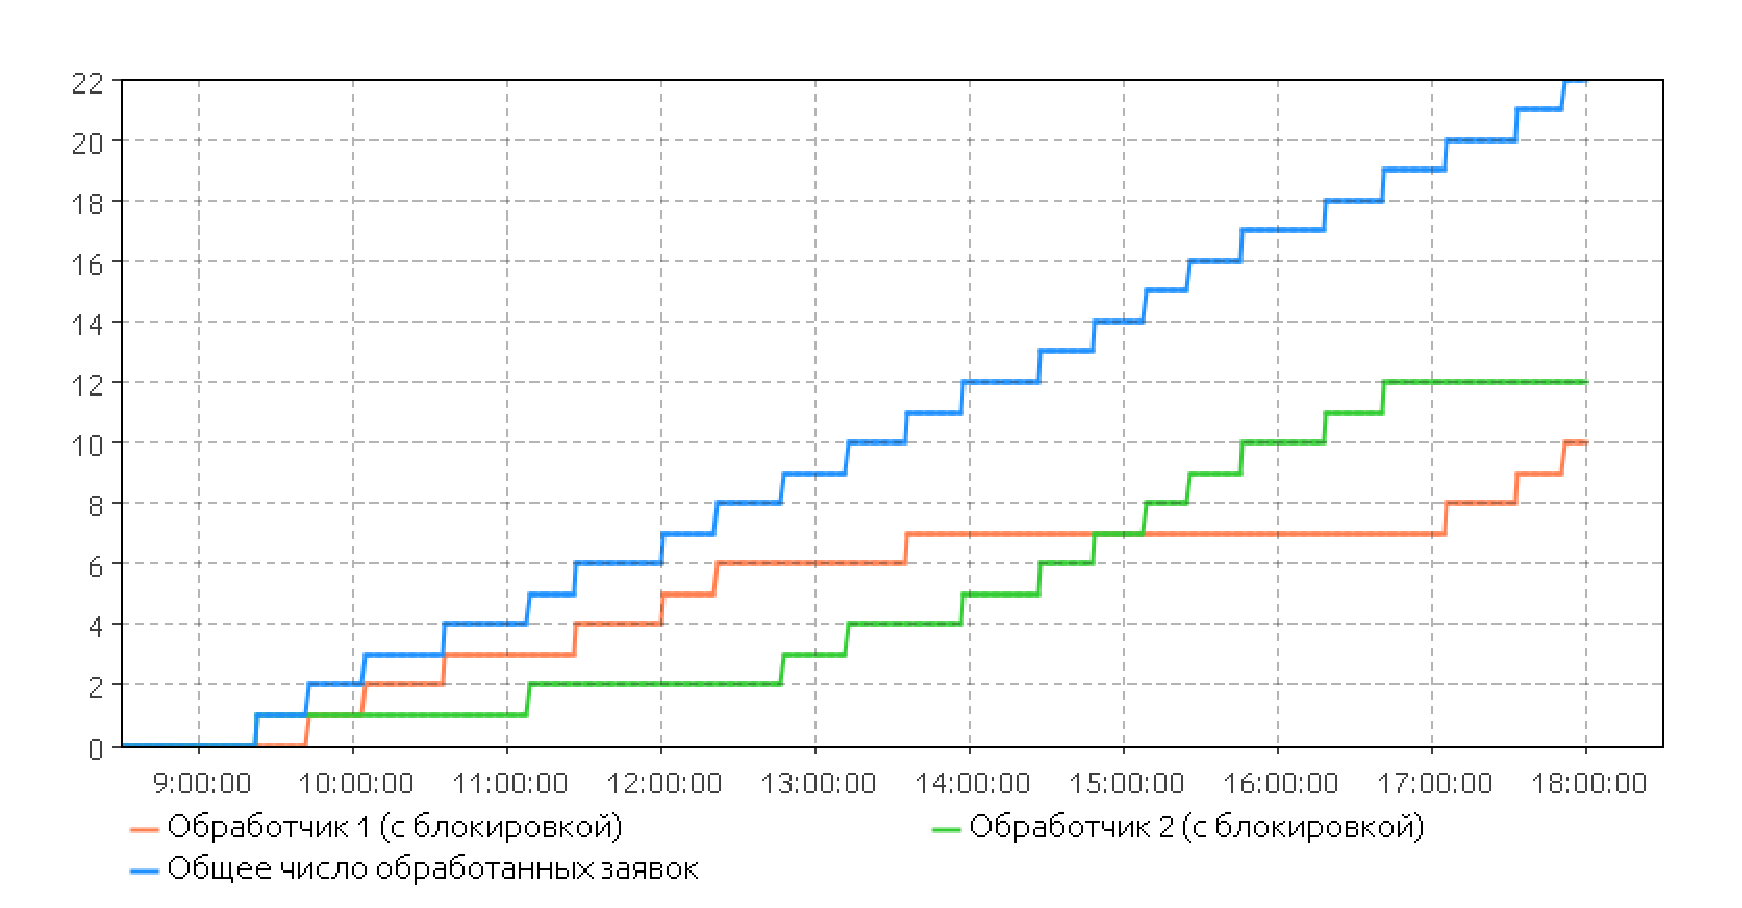
\includegraphics[width=1\textwidth]{competition_old_done}
  \caption{Число обработанных заявок в схеме с блокировкой}
  \label{img:competition_old_done}
\end{figure}

\begin{figure}[h!]
  \centering
  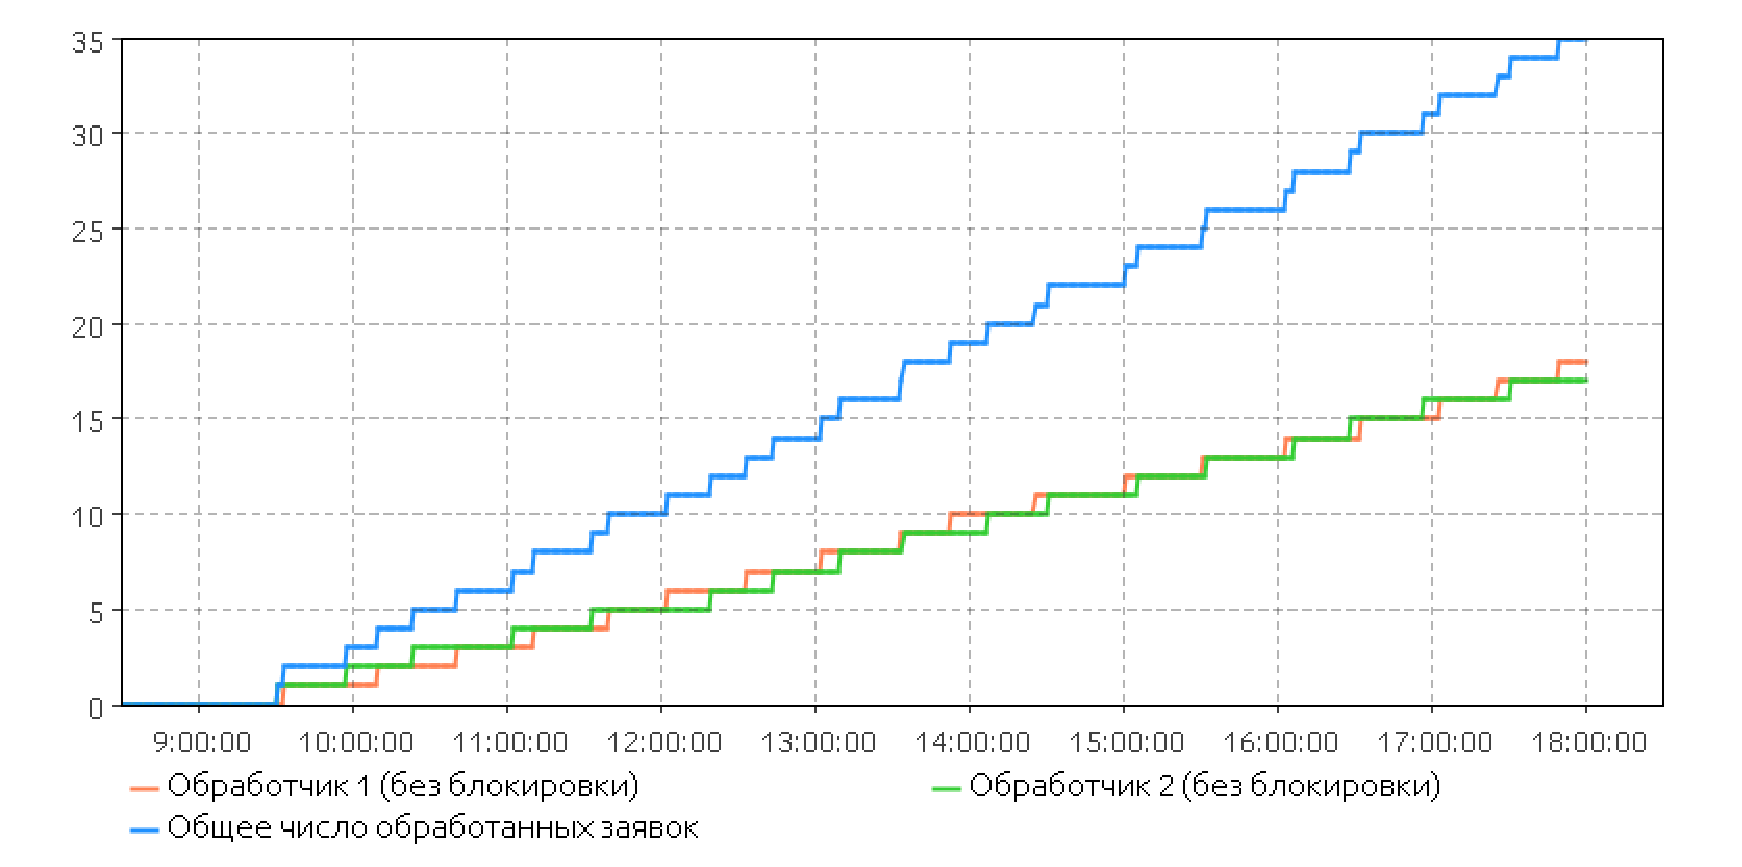
\includegraphics[width=1\textwidth]{competition_new_done}
  \caption{Число обработанных заявок в схеме без блокировки}
  \label{img:competition_new_done}
\end{figure}

\vspace{\baselineskip}
Как видно из представленных результатов, несмотря на б\'{о}льшее среднее время обработки одной заявки число успешно обработанных заявок в схеме без блокировки за один рабочий день в $~1.5$ раза больше, чем число успешно обработанных заявок в схеме с блокировкой за тот же период. Также по этим рисункам видно, что за счёт блокировок заявки в первой схеме обрабатывались неравномерно, в отличие от второй схемы. Дополнительным подтверждением этому служат временн\'{ы}е диаграммы загруженности редакторов в течение рабочего дня, представленные на рис. \ref{img:competition_old_gantt} и \ref{img:competition_new_gantt}.

\begin{figure}[h!]
  \centering
  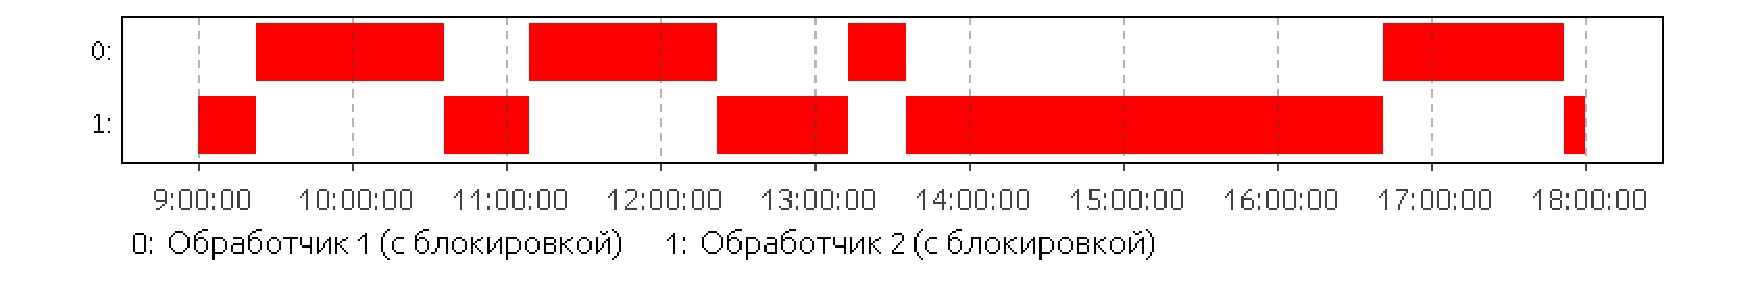
\includegraphics[width=1\textwidth]{competition_old_gantt}
  \caption{Временная диаграмма загруженности редакторов в течение рабочего дня в схеме с блокировкой}
  \label{img:competition_old_gantt}
\end{figure}

\begin{figure}[h!]
  \centering
  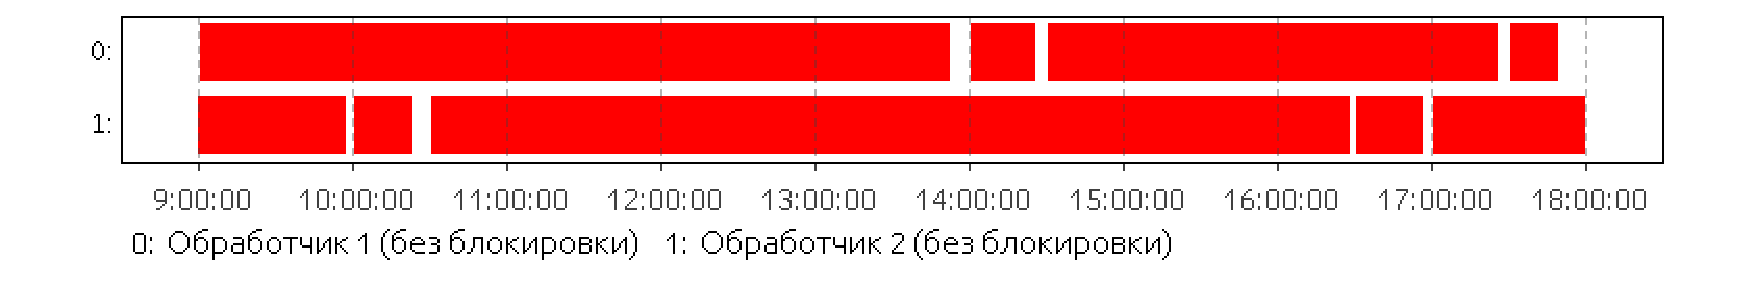
\includegraphics[width=1\textwidth]{competition_new_gantt}
  \caption{Временная диаграмма загруженности редакторов в течение рабочего дня в схеме без блокировки}
  \label{img:competition_new_gantt}
\end{figure}

\vspace{\baselineskip}
Данные рисунки наглядно показывают время бездействия редакторов в схеме с блокировкой (два редактора работают с загрузкой, равной 100\% загрузке одного редактора). Такого продолжительного простоя можно избежать только обрабатывая параллельно несколько документов разными редакторами так, чтобы время блокировок сводилось к минимуму. Таким образом, появляется дополнительная задача временн\'{о}го планирования. При этом схема без блокировок помогает эффективно использовать рабочее время без дополнительного планирования.

\vspace{\baselineskip}
Ещё один немаловажный показатель --- загруженность очереди на обработку. Соответствующие графики приведены на рис. \ref{img:competition_old_queue} и \ref{img:competition_new_queue}.

\begin{figure}[h!]
  \centering
  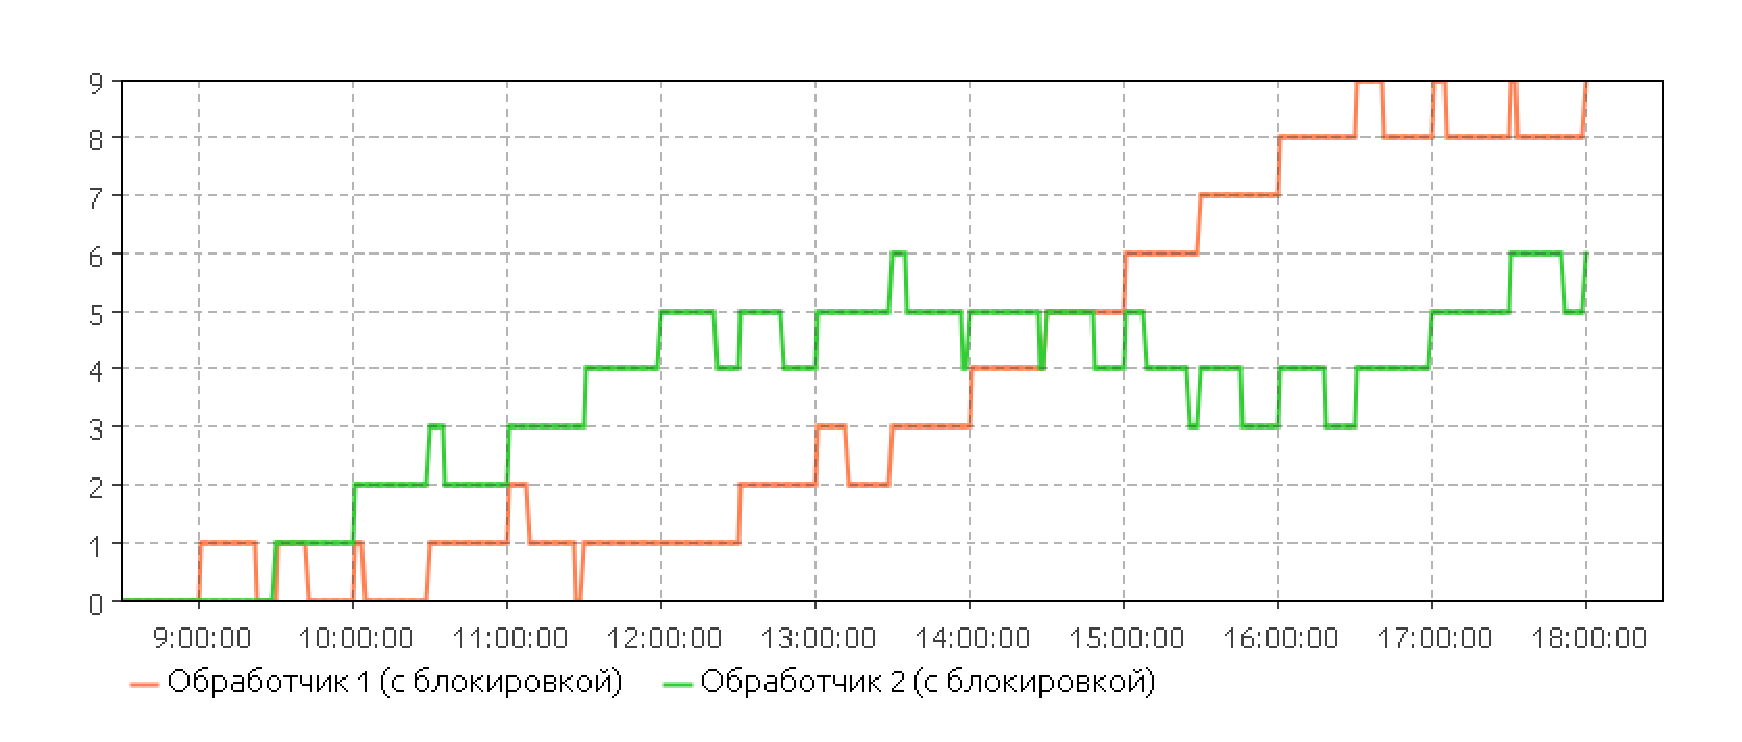
\includegraphics[width=1\textwidth]{competition_old_queue}
  \caption{Загруженность очереди на обработку в схеме с блокировкой}
  \label{img:competition_old_queue}
\end{figure}

\begin{figure}[h!]
  \centering
  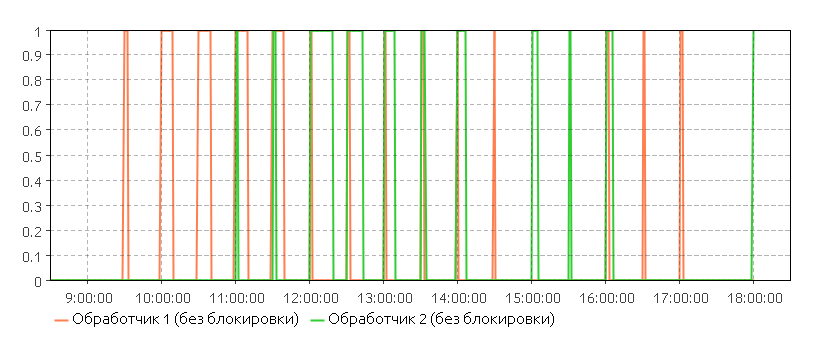
\includegraphics[width=1\textwidth]{competition_new_queue}
  \caption{Загруженность очереди на обработку в схеме без блокировки}
  \label{img:competition_new_queue}
\end{figure}

\vspace{\baselineskip}
Как видно, при использовании схемы с блокировкой заполняемость очереди имеет тенденцию к росту, что в конечном итоге приведёт к ситуации, в которой заявки одного конкретного редактора будут полностью удовлетворены только по завершении всех работ остальными редакторами. В то же время, очереди в схеме без блокировок не имеют подобной тенденции и заявки, находящиеся в них, своевременно удовлетворяются.

\vspace{\baselineskip}
Таким образом, при совместной работе пользователей над одним документом в системе электронного документооборота целесообразно использовать предложенную схему организации процесса без блокировок.			% Конкурентная обработка документа
\subsection{Модуль хранения истории} \label{research_history}

Одной из важных функций системы электронного документооборота и КХЭД как её части является хранение истории внесённых изменений. Это необходимо не только для учёта затраченного времени, но и для разбора конфликтных ситуаций, а также возможности создавать несколько документов на базе одного. Необходимость хранения полной и достоверной истории изменения документа описана в ГОСТ Р ИСО 15489-1 --- 2007 (см. главу \ref{rights_gost_15489_1}). Однако, как показало исследование \ref{review_products}, компании-разработчики СЭД не афишируют способы организации хранения истории, либо полностью полагаются на средства СУБД в части обеспечения целостности данных.

\vspace{\baselineskip}
В общем случае, при таком подходе каждая запись в истории хранится в виде автономного объекта, к которому необходимо добавлять метку времени для упорядочивания событий во временн\textit{о}м порядке и электронную подпись для установления авторства.

\vspace{\baselineskip}
В качестве альтернативы предлагается другой способ хранения истории изменений -- в виде цепочки хэш-сумм. В такой структуре каждая запись содержит в себе контрольную сумма (хэш-сумму) предыдущей записи. Таким образом, события связываются в порядке появления, что избавляет от необходимости дополнительно устанавливать отношения между ними. Дополнительным преимуществом такой схемы является сложность её подделки: если в случае атомарных записей злоумышленник атакует одну целевую запись, то в случае цепочки помимо атаки на целевую запись необходимо также подделать все записи, появившиеся после неё, чтобы целостность цепи не была нарушена. Сложность такой атаки возрастает с увеличением длины цепи.

\vspace{\baselineskip}
В случае дополнения каждой записи электронной подписью, становится возможным просматривать документ с построчным указанием авторства, как показано на рис. \ref{img:git_blame}.

\begin{figure}[h!]
  \centering
  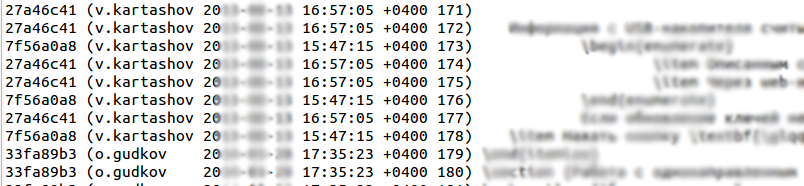
\includegraphics[width=1\textwidth]{git_blame}
  \caption{Просмотр документа с построчным указанием авторства}
  \label{img:git_blame}
\end{figure}

\vspace{\baselineskip}
Таким образом, для проверки целостности истории в первом случае необходимо проверить метку времени каждой записи, а во втором -- лишь убедиться в совпадении соответствующих хэш-сумм. Если последняя операция может считаться атомарной в соответствии с ГОСТ Р 34.11, то проверка метки времени состоит как минимум из трёх операций: сверки хэш-суммы, проверки электронной подписи сервера доверенного времени и проверки электронной подписи удостоверяющего центра, выдавшего сертификат серверу доверенного времени.

\vspace{\baselineskip}
Однако, замеры реализации данных функций средствами openssl не показали большой разницы в результатах: $0.03$ сек. для подсчёта контрольной суммы и $0.05$ сек. для проверки метки времени того же объекта. Это можно объяснить тем, что все операции, необходимые для проверки метки времени, являются независимыми и могут выполняться параллельно.

\vspace{\baselineskip}
Для проверки целостности истории, содержащей 800 записей, в соответствии с описанными замерами была построена схема для имитационного моделирования. Результаты временных замеров представлены на рис. \ref{img:historycheck_time}.

\begin{figure}[h!]
  \centering
  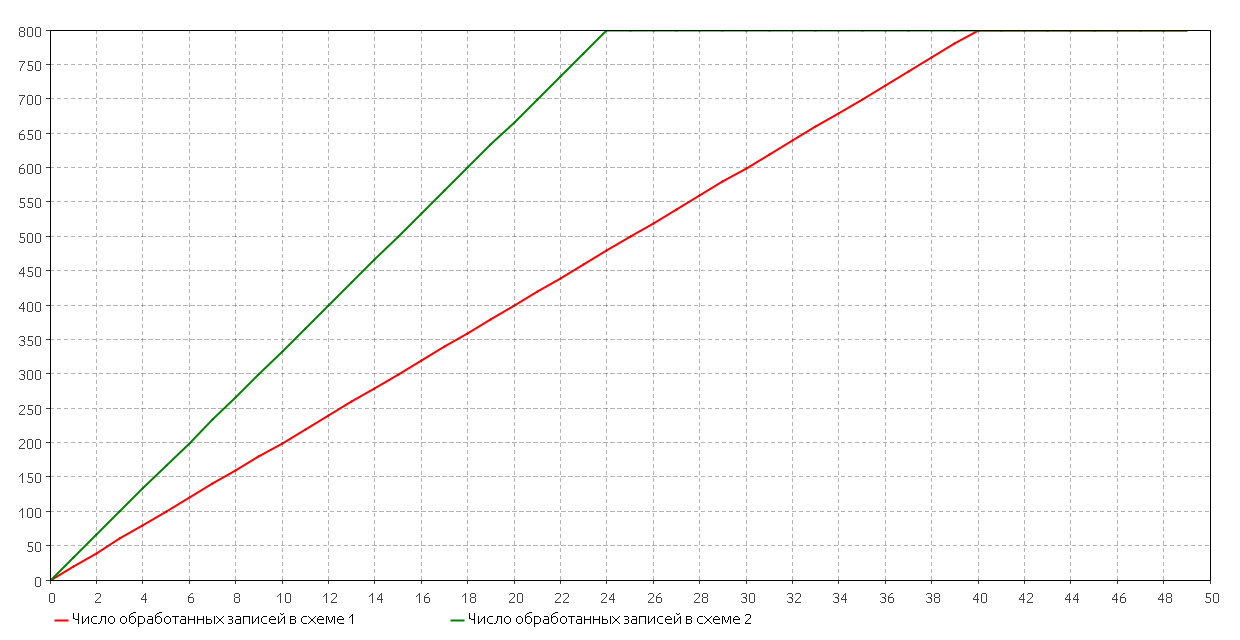
\includegraphics[width=1\textwidth]{historycheck_time}
  \caption{Время проверки целостности истории из 800 записей}
  \label{img:historycheck_time}
\end{figure}

\vspace{\baselineskip}
Как показал эксперимент, даже на таком большом объёме данных использование цепочки хэш-сумм не даёт ощутимого временн\textit{о}го преимущества. Однако, описанный метод имеет другие достоинства: возрастающая с увеличением длины цепочки сложность подделки записей, отсутствие необходимости в содержании сервера доверенного времени. Это позволяет говорить о целесообразности применения такого метода для хранения полной и достоверной истории сделанных изменений.				% Хранение истории